%% NSysS 2026 — full paper submission
%% ACM sigconf. DOUBLE-BLIND: the `anonymous` option is load-bearing. Do not remove it,
%% do not add \acks, and do not name the artefact or link a repository anywhere.
\documentclass[sigconf,anonymous]{acmart}

\usepackage{booktabs}
\usepackage{tikz}
\usepackage{pgfplots}
\pgfplotsset{compat=1.18}

%% One palette for every figure. Chosen to stay legible in greyscale print, which is
%% how a reviewer is most likely to read it: the three series differ in lightness, not
%% only in hue, and every series also carries a distinct mark.
\definecolor{jbInk}{HTML}{1F2933}
\definecolor{jbBlue}{HTML}{2C6E9B}
\definecolor{jbTeal}{HTML}{3F8F7A}
\definecolor{jbAmber}{HTML}{C6873B}
\definecolor{jbRose}{HTML}{A8465F}
\definecolor{jbMist}{HTML}{DDE3E8}
\usetikzlibrary{arrows.meta,positioning,fit,backgrounds,calc,decorations.pathreplacing}

%% Capability glyphs. Math-mode rather than wasysym (which redefines glyphs acmart also
%% defines) and rather than TikZ (which breaks inside \caption, a moving argument).
\newcommand{\CIRCLE}{\ensuremath{\bullet}}
\newcommand{\LEFTcircle}{\ensuremath{\odot}}
\newcommand{\Circle}{\ensuremath{\circ}}

%% Tighter float separation. The paper carries seven floats; acmart's defaults leave more
%% air around each than a two-column layout of this density needs.
\setlength{\textfloatsep}{9pt plus 2pt minus 2pt}
\setlength{\floatsep}{9pt plus 2pt minus 2pt}
\setlength{\intextsep}{9pt plus 2pt minus 2pt}

\settopmatter{printacmref=false}
\renewcommand\footnotetextcopyrightpermission[1]{}
\pagestyle{plain}

\AtBeginDocument{%
  \providecommand\BibTeX{{\normalfont B\kern-0.5em{\scshape i\kern-0.25em b}\kern-0.8em\TeX}}}
\setcopyright{none}
\acmConference[NSysS 2026]{The 13th International Conference on Next-generation
  Computing, Communication, Systems and Security}{December 17--19,
  2026}{Cox's Bazar, Bangladesh}
\acmYear{2026}
\copyrightyear{2026}

\begin{document}

\title{Islands of Reach: A Censorship-Resistant Federated Forum for
National Internet Blackouts}

%% ── AUTHORS ────────────────────────────────────────────────────────────────
%% SUPPRESSED IN SUBMISSION. The `anonymous` option on \documentclass replaces this
%% entire block with "Anonymous Author(s)". Verify with:
%%     pdftotext main.pdf - | grep -i zihad     -> must print nothing
%% For the camera-ready, delete `anonymous` from \documentclass.
\author{Tasmir Hossain Zihad}
\affiliation{%
  \institution{Khulna University of Engineering \& Technology}
  \department{Department of Computer Science and Engineering}
  \city{Khulna}
  \country{Bangladesh}}

\author{Sarwad Hasan Siddiqui}
\affiliation{%
  \institution{Khulna University of Engineering \& Technology}
  \department{Department of Computer Science and Engineering}
  \city{Khulna}
  \country{Bangladesh}}

\author{Rezuan Mustafa Hasan}
\affiliation{%
  \institution{Khulna University of Engineering \& Technology}
  \department{Department of Computer Science and Engineering}
  \city{Khulna}
  \country{Bangladesh}}

\begin{abstract}
A national internet shutdown does not arrive as one event. During the 2024 disruption in Bangladesh,
people met throttling, then blocked platforms, then interference with TLS handshakes, and finally a
five-day blackout. The four major circumvention designs we examine retain a path to infrastructure
outside the censored region; a full transit cut removes that path. We present a public forum ---
communities, posts, threaded comments, votes and moderation, under pseudonymous identities --- built
so that the loss of international transit degrades its reach without ending it. Independent instances
federate directly, and where even domestic peering is cut, a node holding transit on two ISPs bridges
the resulting islands. Every mutation is a signed envelope that carries its own proof of authenticity
and receives the same verification whatever transport delivered it, so trusting a
peer raises how much it may send and never whether what it sends is valid. Content is valid the
instant its author signs it, which removes withheld approval as a censorship mechanism; admission cost
is charged at the origin, because an anti-abuse secret held by one node is meaningless at another; and
spam is priced rather than policed by identity, because requiring identity to stop spam hands the
adversary the lever it wants. We evaluate on a container testbed with independent datastores and
separate address spaces, reporting multi-hop propagation, bridged crossing latency under a severed
exchange, a measured denial-of-service surface, resident memory against a single-board-computer
budget, and encoded size against a measured JSON-LD federation baseline. We also report an
availability defect that only a deployed multi-peer testbed could expose: one unreachable peer stalled
delivery to every reachable one, costing 407\,s per crossing until we isolated and bounded it.
\end{abstract}

\begin{CCSXML}
<ccs2012>
<concept><concept_id>10003033.10003106.10003113</concept_id>
<concept_desc>Networks~Network reliability</concept_desc>
<concept_significance>500</concept_significance></concept>
<concept><concept_id>10002978.10003014.10003017</concept_id>
<concept_desc>Security and privacy~Distributed systems security</concept_desc>
<concept_significance>300</concept_significance></concept>
</ccs2012>
\end{CCSXML}
\ccsdesc[500]{Networks~Network reliability}
\ccsdesc[300]{Security and privacy~Distributed systems security}

\keywords{censorship resistance, internet shutdowns, federation, pseudonymous
publishing, network partitions, transparency logs, canonical encoding}

\maketitle

%% ────────────────────────────────────────────────────────────────────────────
\section{Introduction}
\label{sec:intro}

Internet shutdowns are usually described as on or off. They are not. The record of the July--August
2024 disruption in Bangladesh is a sequence of separate technical
conditions~\cite{ooni2025bangladesh}: selective throttling, blocking of individual platforms,
interference with TLS handshakes, and then a national blackout lasting five days. Each condition
breaks a different assumption, and a tool that handles one can fail completely at the next. How the
blackout was produced matters for what can survive it: the broadband cut was executed upstream,
through instructions issued to international terrestrial cable operators, the submarine cable company
and IIG providers~\cite{ooni2025bangladesh}, so what was withdrawn was the country's transit rather
than its internal networks. Shutdowns of this shape are not rare enough to treat as an edge
case~\cite{bischof2023shutdowns}.

What people lose in that sequence is not only messaging. It is the ability to publish to strangers:
to say what is happening in a place, to be read by people who were not already in your contact list,
and to have what you said remain checkable afterwards. That is a forum, and a forum is harder to keep
alive under a shutdown than a chat application, because it needs durable content, a notion of
community, moderation that is not itself a censorship lever, and identities that are recognisable
without being attributable.

We name the conditions as rungs of a ladder. \textbf{L0} is unimpeded global reach. \textbf{L1} is a
national partition: hosts inside the country can reach each other but not the outside. \textbf{L2} is
an ISP island, where even domestic peering is severed and a network reaches only its own subscribers.
\textbf{L3} is two or more such islands rejoined by an operator that holds transit on both.
Figure~\ref{fig:ladder} summarises the ladder. The system needs an IP path; what it does not need is
an \emph{unfiltered} one, or one that leaves the country.

\textbf{Scope.} We make no claim below L3. The repository also contains a separate identified
emergency-communication plane, local WebRTC exchange, portable offline bundles and an optional
Reticulum adapter. They are product features, not evidence for the result reported here. Off-grid
mesh, Bluetooth relaying and long-range radio are a different problem with a different literature,
and nothing in this paper depends on them. Tor access is discussed separately because it can help
under selective blocking, but it still needs a reachable Tor path and therefore cannot establish the
L1--L3 claim.

\begin{figure}[t]
\centering
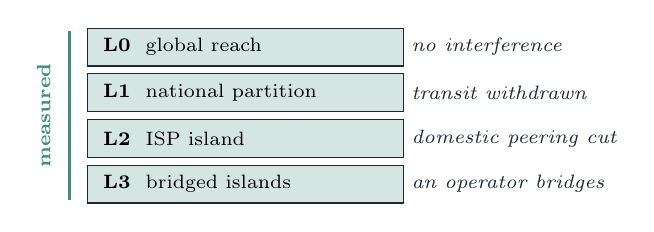
\begin{tikzpicture}[
  font=\scriptsize,
  rung/.style={draw=jbInk,line width=0.4pt,minimum height=4.8mm,inner xsep=3pt,anchor=west},
  ours/.style={rung,fill=jbTeal!22},
  lbl/.style={font=\scriptsize\itshape,anchor=west,text=jbInk}
]
\def\W{38mm}
\foreach \i/\name/\what in {
  0/L0/global reach,
  1/L1/national partition,
  2/L2/ISP island,
  3/L3/bridged islands}
{
  \node[ours,minimum width=\W] (r\i) at (0,{-\i*5.8mm}) {\makebox[\W][l]{\ \textbf{\name}\ \ \what}};
}
\node[lbl] at (40mm,0)        {no interference};
\node[lbl] at (40mm,-5.8mm)   {transit withdrawn};
\node[lbl] at (40mm,-11.6mm)  {domestic peering cut};
\node[lbl] at (40mm,-17.4mm)  {an operator bridges};
\draw[jbTeal,line width=1pt] (-2.2mm,2mm) -- (-2.2mm,-19.4mm);
\node[rotate=90,anchor=south,font=\scriptsize\bfseries,text=jbTeal]
  at (-3.4mm,-8.7mm) {measured};
\end{tikzpicture}
\caption{The resilience ladder. A different action cuts each rung, and a tool that survives one can
fail entirely at the next. Circumvention systems require some remaining L0 path to infrastructure
outside the censor; common federated social systems also assume global reach. We measure
L0--L3.}
\label{fig:ladder}
\Description{Four reachability levels from ordinary connectivity through a national transit cut, an
ISP island and two ISP islands joined by a multi-homed bridge.}
\end{figure}

The gap we address is that the two families of systems built for exactly this adversary both stop at
L1, and for the same reason. \emph{Circumvention} systems --- Tor's blocking-resistant
design~\cite{torblocking2006}, domain fronting~\cite{fifield2015fronting},
decoy routing~\cite{wustrow2011telex}, Snowflake~\cite{bocovich2024snowflake} --- each work by
reaching something the censor does not control, which is a host outside the censored region. Telex
says so outright: governments that "disconnect entirely in times of crisis'' are "outside our threat
model''~\cite{wustrow2011telex}. \emph{Federated} social systems --- ActivityPub~\cite{activitypub},
Matrix~\cite{matrixspec}, the AT Protocol~\cite{atproto} --- assume L0 and define federation as
delivery to a named remote host, and their reachability is more brittle than the architecture
suggests: removing instances hosted in five autonomous systems from Mastodon's measured graph cuts
its largest connected component from 92\% of users to 46\%~\cite{raman2019mastodon}. A population under a national blackout needs the rungs below
L1, and that is where neither family operates.

We should say at the outset that the \emph{mechanisms} we use are not new. Addressing content by the
hash of its canonical encoding and signing it at rest is Nostr~\cite{nostr} and Secure
Scuttlebutt~\cite{tarr2019ssb}. Gossiping tree heads to detect a rewritten log is Certificate
Transparency~\cite{rfc6962}. Separating credential issuance from credential verification is Privacy
Pass~\cite{davidson2018privacypass}. Preferring the narrowest working path while keeping alternates
warm is ICE~\cite{rfc8445} and MPTCP~\cite{rfc8684}. What we contribute is the composition, the
invariants that composition forces on us, and what it costs once measured.

\noindent This paper contributes:

\begin{itemize}
  \item \textbf{Canonicalisation as an \emph{admission} test, and the three-position design space it
    completes.} Prior systems either canonicalise inside the verifier (Matrix) or refuse to define a
    canonical form at all (Cosmos SDK). These are two of three positions. We take the third, and it
    buys a property we can state plainly: no canonicalisation function ever sits between an attacker
    and a verifier, so a relay that re-encodes a message cannot quietly \emph{repair} a malformed
    object into a verifiable one (\S\ref{sec:canonical}).
  \item \textbf{A conservative fork policy when no consistency proof can be fetched.} The CT
    gossip literature settles an ambiguous pair of tree heads with a consistency proof, and fetching
    one costs a round trip to the peer whose reachability is already in doubt. That makes it
    unavailable during a partition, which is when fork detection is most likely to fire. We show that
    the resulting false accusations are real and severe (one uplink flap wrongly blocked two of three
    honest peers), give a weaker local rule that avoids that false positive without a round trip, and
    state explicitly that it neither proves consistency nor identifies an honest branch
    (\S\ref{sec:fork}).
  \item \textbf{Two federation invariants, each stated with the deployed failure that produced it.}
    An identifier inside a federated payload has to be derivable by any node from the signed bytes,
    and admission cost has to be charged at the origin, because a node's local anti-abuse secrets mean
    nothing anywhere else (\S\ref{sec:federation}).
  \item \textbf{A partition testbed, a resilience ladder that makes such systems comparable, and the
    first measurements of this one:} propagation measured over hop count and queueing parameter, an
    island crossing under a severed exchange, resident memory against a single-board-computer budget,
    encoded size against a measured ActivityPub baseline, and a denial-of-service surface measured
    rather than asserted (\S\ref{sec:eval}).
\end{itemize}

%% ---------------------------------------------------------------------------
\section{Related Work}
\label{sec:related}

This venue spans networking and security broadly, so we introduce each concept instead of assuming
it.

\paragraph{Censorship-resistant publishing.} The problem is not new, and neither is our adversary.
Publius~\cite{waldman2000publius} splits a document across servers so no single operator can remove
it; Freenet~\cite{clarke2001freenet} makes stored content unidentifiable to the node storing it;
Tangler~\cite{waldman2001tangler} entangles blocks so a server has reason to keep any particular one.
What unites them is the threat they solve, \emph{takedown of the hosts}, and the remedy they reach
for, \emph{geography}. Tangler names our attack exactly --- "an attack with the same end result is to
simply force the hosting servers off the network so that potential readers cannot contact the
servers'' --- and answers it by replicating across "many different countries and judicial
domains''~\cite{waldman2001tangler}. That answer requires the reader to reach those countries. It
resolves a takedown and does nothing for a blackout, and closing that gap is what this paper is for.
The circumvention systems named in \S\ref{sec:intro} share the same dependency and say so
themselves~\cite{torblocking2006,fifield2015fronting,wustrow2011telex,bocovich2024snowflake}.

\paragraph{Federated public discussion.} Netnews is the historical baseline: independent servers
relay topic-grouped public articles, retry transfers and apply local moderation and acceptance
policy~\cite{rfc5537}. Its base format does not authenticate authors. Nostr~\cite{nostr} and
Secure Scuttlebutt~\cite{tarr2019ssb,ssbprotocolguide} instead use author-signed objects that readers
verify without a server. SSB replicates among addressable peers; base Nostr has no relay-to-relay
exchange, although a client can copy events and draft NIP-77 defines optional reconciliation
~\cite{nostrnip77}. None specifies our scope-aware multi-ISP availability policy.

\paragraph{Federation over IP.} ActivityPub~\cite{activitypub} is the dominant federation protocol
and makes neither object signatures nor HTTP Signatures normative; its authentication discussion sits
in a non-normative appendix. Matrix~\cite{matrixspec} signs events over a Canonical JSON form,
and has been analysed adversarially~\cite{albrecht2023matrix}. The AT Protocol~\cite{atproto} is the
closest prior composition to ours --- signed commits over a Merkle search tree with deterministic
CBOR --- but its verification depends on an external identity directory operated by a single
company~\cite{balduf2024bluesky}, which a shutdown removes. Decentralised moderation in these systems
is itself a studied problem~\cite{anaobi2023moderation}, and it shapes our decision to make
moderation additive rather than gatekeeping.

\paragraph{Transparency logs.} Certificate Transparency~\cite{rfc6962} established the pattern we
reuse: an append-only Merkle log~\cite{merkle1988} whose signed tree heads are gossiped, so anyone
comparing two heads can detect a participant that rewrote history. Comparing heads safely is itself
well studied~\cite{dahlberg2018aggregation,rfc9162}, and every applicable
resolution needs a consistency proof. \S\ref{sec:fork} is about the window in which that proof cannot
be fetched.

\paragraph{Anti-abuse without identity.} Pricing admission rather than checking
identity~\cite{dworknaor1993pricing}, blind signatures~\cite{chaum1983blind} and their modern
deployment as Privacy Pass~\cite{davidson2018privacypass,rfc9576} let a system charge an anonymous
participant. We adopt this because the alternative is worse than inconvenient: the UN Special
Rapporteur's finding is that identity requirements are themselves a restriction on
expression~\cite{unhrc2015anonymity}, so an anti-abuse design that demands identity hands the
adversary the lever it wants.

\paragraph{Path selection.} ICE~\cite{rfc8445} and MPTCP~\cite{rfc8684} show that holding several
candidate paths and continuously preferring among them beats failing over on demand. We apply the
same reasoning to reachability \emph{scope} rather than to addresses.

%% ---
%% ---------------------------------------------------------------------------
\section{Design}
\label{sec:design}
\subsection{One write path}

The system exposes exactly one write endpoint. A post, a vote, a moderation action, a key revocation
and a broadcast are all the same structure: an \emph{envelope} carrying a domain string, an author
key, a timestamp, a priority class, an opaque body and a signature. There is no per-feature write
route. Adding a feature adds a registry row and a handler, not a branch anywhere in the ingress path.

The envelope's identifier comes from its own bytes:
\[
\textit{id} = \textsc{base32}\big(\textsc{sha-256}(\textit{canonical}(\textit{fields}_{1..12}))\big)
\]
and the Ed25519~\cite{bernstein2012ed25519} signature covers those same bytes. Nothing in this
identifier depends on which node computed it, which is what lets two independent instances agree on
identity without coordinating.

The Forum registry covers communities, memberships, posts, threaded comments, votes, attachments,
profiles, social actions, pseudonymous messages and signed moderation records. The same codebase has
a separate Signal plane for identified channels, ordered emergency broadcasts, check-ins, crisis
reports and encrypted messages. Plane-scoped certificates prevent a Forum pseudonym from
authorising a Signal action. This paper evaluates the Forum plane; the Signal feature set is stated
here to define the system boundary, not to enlarge the evaluation claim.

\subsection{Canonical encoding as an admission gate}
\label{sec:canonical}

Matrix re-encodes parsed events as Canonical JSON and verifies that result~\cite{matrixspec}; Cosmos
instead verifies received protobuf bytes and rejects a canonicalisation requirement as extra client
complexity that restricts upgrades~\cite{cosmosadr020}. We combine a defined form with the latter's
verification rule, but order them differently. Before verification, the decoder re-encodes the parsed
message and rejects any mismatch. The signature is then checked against \textbf{the bytes as they
arrived}, never against repaired bytes. Canonicalisation therefore decides what to admit, not what to
verify against.

This prevents a relay from turning a malformed encoding into a valid-looking object by re-serialising
it. Protobuf itself is not canonical~\cite{protobufnotcanonical}, so our profile defines one accepted
form and proves it across implementations (\S\ref{sec:eval-vectors}). The cost is explicit: unknown
fields are not retained and compatible evolution needs a version bump.

\subsection{The validation pipeline}

Every envelope, from every transport, runs the same nineteen-step pipeline in the same order
(Figure~\ref{fig:pipeline}). Naming all nineteen matters because two of the orderings are load-bearing
security properties rather than implementation taste, and neither is visible from a summary.

\textbf{Steps 1--12 write nothing to the database.} Everything that can be decided from the bytes and
the local index alone is decided first: size on the raw bytes before parsing, canonical decode,
registry lookup, clock bounds, the signature, the author's certificate, the dedupe index and the
replay check. Only at step 13 does the node touch storage. A flood of invalid envelopes therefore
costs CPU and nothing else, which we measure in \S\ref{sec:flood}.

\textbf{Steps 16 and 17 commit together.} The projection and the Merkle append occur in one
transaction, because an envelope visible in a projection but missing from the log is exactly the
transparency failure the log exists to prevent. This forces a deployment constraint --- the storage
engine must support multi-document transactions --- which we state rather than hide.

\textbf{A federated envelope does not get weaker verification.} Every applicable step re-runs at the
receiver. Step~13 is the sole exception, for a precise reason given in \S\ref{sec:federation}: the
cost was charged at the origin and its proof is keyed to that node, so what is skipped is a payment
and not a check. Each step is a pure function that can be tested on its own.

\begin{figure}[t]
\centering
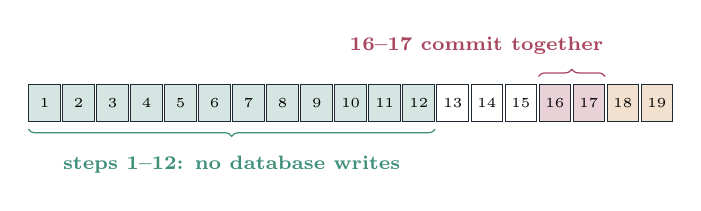
\begin{tikzpicture}[font=\scriptsize,
  cell/.style={draw=jbInk,line width=0.25pt,minimum width=4.05mm,minimum height=4.6mm,
               inner sep=0pt,font=\tiny},
  nw/.style={cell,fill=jbTeal!22},
  mid/.style={cell,fill=white},
  atomicstep/.style={cell,fill=jbRose!25},
  em/.style={cell,fill=jbAmber!25}]
\def\dx{4.32mm}
\foreach \i in {1,...,12}{\node[nw]         (p\i) at ({(\i-1)*\dx},0) {\i};}
\foreach \i in {13,14,15}{\node[mid]        (p\i) at ({(\i-1)*\dx},0) {\i};}
\foreach \i in {16,17}   {\node[atomicstep] (p\i) at ({(\i-1)*\dx},0) {\i};}
\foreach \i in {18,19}   {\node[em]         (p\i) at ({(\i-1)*\dx},0) {\i};}
% no-write prefix, below
\draw[decorate,decoration={brace,amplitude=2.6pt,mirror},jbTeal,line width=0.45pt]
  ($(p1.south west)+(0,-1mm)$) -- ($(p12.south east)+(0,-1mm)$);
\node[font=\scriptsize,text=jbTeal,anchor=north]
  at ($(p1.south west)!0.5!(p12.south east)+(0,-3.2mm)$)
  {\textbf{steps 1--12: no database writes}};
% atomic pair, above
\draw[decorate,decoration={brace,amplitude=2.6pt},jbRose,line width=0.45pt]
  ($(p16.north west)+(0,1mm)$) -- ($(p17.north east)+(0,1mm)$);
\node[font=\scriptsize,text=jbRose,anchor=south east]
  at ($(p17.north east)+(1mm,2.6mm)$) {\textbf{16--17 commit together}};
\end{tikzpicture}
\caption{The nineteen steps, in order.
\emph{1} size, on raw bytes before parsing \textperiodcentered\
\emph{2} parse, canonical decode with unknown fields rejected \textperiodcentered\
\emph{3} version \textperiodcentered\ \emph{4} domain \textperiodcentered\ \emph{5} plane
\textperiodcentered\ \emph{6} algorithm policy \textperiodcentered\ \emph{7} priority
\textperiodcentered\ \emph{8} clock \textperiodcentered\ \emph{9} signature \textperiodcentered\
\emph{10} certificate \textperiodcentered\ \emph{11} dedupe \textperiodcentered\ \emph{12} replay
\textperiodcentered\ \emph{13} anti-abuse \textperiodcentered\ \emph{14} authorise
\textperiodcentered\ \emph{15} body validate \textperiodcentered\ \emph{16} apply
\textperiodcentered\ \emph{17} witness \textperiodcentered\ \emph{18} receipt \textperiodcentered\
\emph{19} fanout. An inbound federated envelope re-runs all of them except 13.}
\label{fig:pipeline}
\Description{Nineteen numbered admission steps. Steps one through twelve perform no database writes,
while steps sixteen and seventeen commit the projection and Merkle witness together.}
\end{figure}

\subsection{The audit-log workflow}
\label{sec:als}

Modification, deletion and omission are different attacks. A signature detects modification but not
whether a server accepted an object. Figure~\ref{fig:write-als} follows one public write. The client
queues the final signed request before sending it. After admission, steps 16--17 commit the projection
and Merkle leaf together; step 18 returns a node-signed receipt with the server and content identities,
leaf position, signed tree head and inclusion proof. The client binds that receipt to the \emph{exact
UTF-8 request body}, verifies the resulting audit certificate and saves it locally first.

The client forwards the certificate to each configured independent audit-log server (ALS). Each ALS
decodes the original envelope, enforces canonical encoding, recomputes its identifiers, verifies the
receipt, tree-head signatures and inclusion proof, then appends it to a JSONL hash chain. Exact retries
are idempotent; conflicting certificates for one $(server,content)$ pair are rejected. Failed
deliveries remain pending, and provenance failures enter a separate hash-chained issue stream.

Later, the client presents the certificate to the \emph{issuing node}'s \texttt{/status} endpoint,
which reports online, hidden, deleted or wrong-server status. The ALS preserves the earlier
acknowledgement; it does not claim current node state. Public certificates may be copied externally,
but direct-message certificates remain local to avoid exposing a timestamped social graph.

\begin{figure*}[t]
\centering
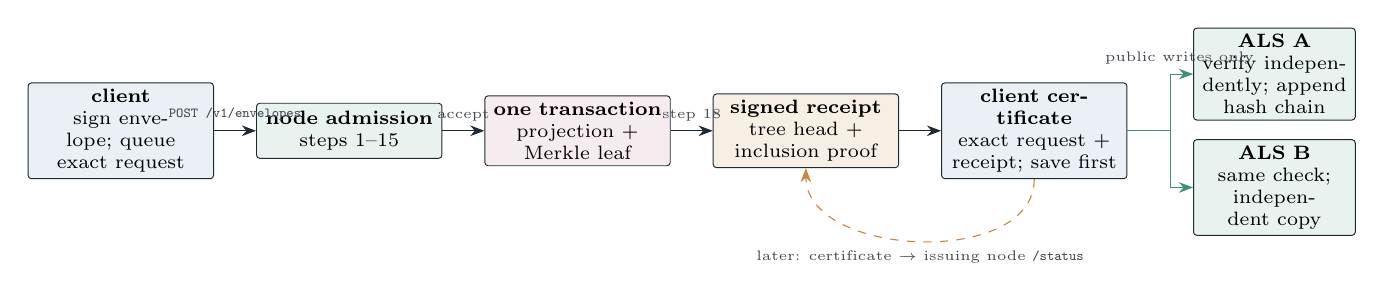
\begin{tikzpicture}[
  font=\scriptsize,
  box/.style={draw=jbInk,line width=0.35pt,rounded corners=1.2pt,minimum height=7mm,
              text width=22mm,align=center,inner sep=2.2pt},
  smallbox/.style={box,text width=19mm},
  note/.style={font=\tiny,align=center,text=jbInk!85},
  >={Stealth[length=1.8mm]}
]
\node[box,fill=jbBlue!10] (client) at (0,0) {\textbf{client}\\sign envelope; queue exact request};
\node[box,fill=jbTeal!12] (pipe) at (2.9,0) {\textbf{node admission}\\steps 1--15};
\node[box,fill=jbRose!10] (commit) at (5.8,0) {\textbf{one transaction}\\projection + Merkle leaf};
\node[box,fill=jbAmber!14] (receipt) at (8.7,0) {\textbf{signed receipt}\\tree head + inclusion proof};
\node[box,fill=jbBlue!10] (cert) at (11.6,0) {\textbf{client certificate}\\exact request + receipt; save first};
\node[smallbox,fill=jbTeal!12] (alsa) at (14.65,0.72) {\textbf{ALS A}\\verify independently; append hash chain};
\node[smallbox,fill=jbTeal!12] (alsb) at (14.65,-0.72) {\textbf{ALS B}\\same check; independent copy};

\draw[->,jbInk] (client) -- node[above,note]{\texttt{POST /v1/envelopes}} (pipe);
\draw[->,jbInk] (pipe) -- node[above,note]{accept} (commit);
\draw[->,jbInk] (commit) -- node[above,note]{step 18} (receipt);
\draw[->,jbInk] (receipt) -- (cert);
\draw[->,jbTeal] (cert.east) -- ++(0.55,0) |- node[pos=0.7,above,note]{public writes only} (alsa.west);
\draw[->,jbTeal] (cert.east) -- ++(0.55,0) |- (alsb.west);
\draw[->,dashed,jbAmber] (cert.south) to[out=-90,in=-90]
  node[below,note]{later: certificate $\rightarrow$ issuing node \texttt{/status}} (receipt.south);
\end{tikzpicture}
\caption{One write path and the ALS workflow. The client keeps the certificate before forwarding it,
so audit delivery can resume after an outage. An ALS verifies a node's prior acknowledgement and
retains it independently; only the issuing node reports whether the content is currently online,
hidden or missing.}
\label{fig:write-als}
\Description{A signed request passes through node validation and an atomic projection and Merkle-log
commit. The node returns a signed receipt. The client stores an audit certificate containing the
exact request and receipt, then forwards public certificates to two independent audit-log servers.}
\end{figure*}

This is evidence, not immutable storage. It proves prior acknowledgement, but cannot prove acceptance
without a receipt, compel service, or recover a body after every copy is destroyed. An ALS can also
withhold its copy; replication helps only when clients and auditors are independent.

\subsection{Additive labels as an open taxonomy}
\label{sec:classify}

Moderation here is already additive: a \texttt{Label} is a signed opinion about content that is
already published, never a precondition for publishing it, and removal leaves a tombstone rather
than an absence. What is easy to miss is that this already holds at the protocol level, not only
as policy. A label's category field is a free string rather than a closed enumeration, its
model or moderator identifier is likewise free text, and an \emph{unscoped} label needs no
community's permission to publish at all --- a third-party fact-checker or community moderation
team writes one exactly as the local instance would, over the same one write path
(\S\ref{sec:design}). No vocabulary and no publishing key is privileged by the protocol.

We take this as evidence that the same mechanism generalises past a single safety verdict. A
node behind a partition benefits from surfacing \emph{who is asking for help} at least as much as
\emph{what should be hidden}, so we specify --- but, in the sense that \S\ref{sec:intro} states the
Signal plane to define the system boundary rather than to enlarge the evaluation claim, do not here
evaluate --- an extension from one closed verdict to open
\texttt{(taxonomy, label, score)} triples covering sentiment, topical intent and language. A
taxonomy this node has never seen before still canonicalises, signs, verifies and federates,
because it is carried as data rather than adopted as protocol; publishing it costs a registry row
and a handler, and the admission path in Figure~\ref{fig:pipeline} gains no new step, because an
assertion is an ordinary envelope through the ordinary path (Figure~\ref{fig:classify}). What
changes for a client is only which taxonomies a given node advertises, over a manifest it is free
to ignore.

Two consequences follow directly from reusing rather than extending the write path, and neither is
specific to sentiment or intent. First, whatever classifier an operator runs cannot gate a post,
because nothing between \S\ref{sec:canonical} and \S\ref{sec:als} consults one; the worst it can do
is answer late or not at all, which is the same failure mode \S\ref{sec:related} already accepts
for any labeller. Second, no one classifier's output is structurally load-bearing: the taxonomy it
speaks is metadata a reader may act on, not a gate a publisher must pass.

\begin{figure}[t]
\centering
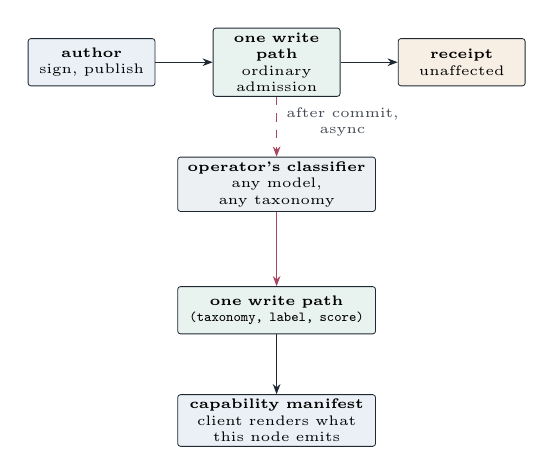
\begin{tikzpicture}[
  font=\tiny,
  box/.style={draw=jbInk,line width=0.3pt,rounded corners=1pt,minimum height=6mm,
              text width=15mm,align=center,inner sep=1.6pt},
  wbox/.style={box,text width=24mm},
  note/.style={font=\tiny,align=center,text=jbInk!85},
  >={Stealth[length=1.3mm]}
]
\node[box,fill=jbBlue!10]  (author) at (0,0)   {\textbf{author}\\sign, publish};
\node[box,fill=jbTeal!12]  (wp1)    at (2.35,0) {\textbf{one write path}\\ordinary admission};
\node[box,fill=jbAmber!14] (rcpt)   at (4.7,0)  {\textbf{receipt}\\unaffected};
\draw[->,jbInk] (author) -- (wp1);
\draw[->,jbInk] (wp1) -- (rcpt);

\node[wbox,fill=jbMist!55] (clf) at (2.35,-1.55)
  {\textbf{operator's classifier}\\any model, any taxonomy};
\draw[->,dashed,jbRose,line width=0.4pt] (wp1.south) --
  node[right,note,pos=0.42]{after commit,\\async} (clf.north);

\node[wbox,fill=jbTeal!12] (wp2) at (2.35,-3.15)
  {\textbf{one write path}\\\texttt{(taxonomy, label, score)}};
\draw[->,jbRose,line width=0.4pt] (clf) -- (wp2);

\node[wbox,fill=jbBlue!10] (manifest) at (2.35,-4.55)
  {\textbf{capability manifest}\\client renders what this node emits};
\draw[->,jbInk] (wp2) -- (manifest);
\end{tikzpicture}
\caption{Publishing is unaffected by classification: the top row is the ordinary write path and
returns its receipt whether or not any classifier ever runs. An accepted post's content ID is
handed to an operator-chosen classifier only afterward and off the critical path; its opinion
re-enters through the same write path as an ordinary envelope, carrying an open taxonomy rather
than a fixed vocabulary, and a capability manifest tells a client which taxonomies this particular
node speaks. This design is specified, not evaluated.}
\label{fig:classify}
\Description{A publish path from author through the one write path to a receipt, unaffected by
classification. A dashed arrow leaves the write path after commit toward an operator-chosen
classifier, whose opinion re-enters through the same write path as an open taxonomy triple and
is exposed to clients through a capability manifest.}
\end{figure}


%% ---------------------------------------------------------------------------
\section{Federating Across a Partition}
\label{sec:federation}
Federation is server to server only. Clients do not speak it, because operators choose their peers
and clients do not, and because the protocol's connection profile degrades badly on lossy mobile
links.

The ISP subsystem is separate from the nineteen admission steps. Its 22 implementation tasks cover
four groups: scoped endpoints, probes, source binding, ranking, backoff and metrics; durable peer and
seed discovery plus local/manual discovery and NAT traversal; opt-in bridge relay, reserved quotas,
uplink failover, re-announcement and backfill; and client/operator visibility. Bridging itself is not
a twentieth verifier: it is the policy attached to step~19, after the received envelope has passed
the same applicable admission checks as a local one.

\subsection{Four rules that carry the weight}

\paragraph{Peer bytes are never re-encoded.} The transport uses a passthrough codec. The decoder
establishes canonicality by re-encoding and comparing (\S\ref{sec:canonical}), so a round trip through
a generated codec inside the network adapter would quietly repair an untrusted peer's non-canonical
envelope into one that validates. That is the exact hazard the admission gate exists to stop, arriving
over the network and going around it.

\paragraph{Trust bounds volume, never validity.} Inbound envelopes re-run every applicable step. A
trusted peer's forged envelope is rejected exactly as a stranger's is. Trust sets the quota and the
priority classes a peer may push, and nothing else.

\paragraph{Deduplication is a unique index, not a read-then-write.} The pair
$(\textit{content\_id}, \textit{direction})$ is a uniqueness constraint in the database. A read-then-write check is unsound
under the concurrency federation produces, where an overlapping stream and a backfill can deliver the
same envelope twice at once.

\paragraph{An envelope is never relayed to its sender.} The pipeline carries the origin peer and
excludes it from fanout. Content dedupe makes such a loop terminate, but it does not make it free:
without this rule, every envelope pays a round trip before being thrown away.

\subsection{Two invariants, and the failures that produced them}

\paragraph{An identifier in a federated payload has to be derivable from the signed bytes.} An earlier
version derived a community identifier from the projecting node's own key. With one node that is
indistinguishable from correct, because the projecting node \emph{is} the origin node. With two, the
same signed envelope produced a different community identifier on each instance, and the projections
diverged for good. The rule that replaced it is a question asked before any identifier is minted:
\emph{would a different node, given only these bytes, compute the same value?}

\paragraph{Admission cost is charged at the origin.} Proof-of-work, credit balances, blind credentials
and epoch nullifiers are each deliberately keyed to one node. A proof minted at the origin is
therefore not merely unverifiable elsewhere, it is meaningless elsewhere. Charging again on receipt
would make every anti-abuse-gated domain impossible to federate. Cost is paid once, at the origin, and
the receiver's protection is a per-peer, per-class quota with an explicit backpressure hint.
Verification is untouched: what is skipped is a payment, not a check.

One consequence is that a peer over quota is not disconnected. It would reconnect immediately, pay the
handshake again and arrive in the same state, so refusing costs more than accepting. The hint lets a
well-behaved peer slow itself down, and a peer that ignores the hint is demoted.

\subsection{Federating from a node nothing can dial}
\label{sec:cgnat}

In ActivityPub, Matrix and the AT Protocol, server-to-server delivery is a \emph{push to an address
the receiver publishes}, so a node with no inbound reachability cannot receive at all unless a third
party holds an address for it. In the deployments this paper is about, that is the common case rather
than the corner case: a community node is a machine in somebody's home, behind carrier-grade NAT. We
make reachability an asymmetry instead of a requirement, so a node may advertise \emph{no} endpoints
and still federate both ways:

\begin{itemize}\itemsep1pt
  \item \textbf{outbound} is the durable outbox draining over a connection the node opened;
  \item \textbf{inbound} is a resumable backfill the node \emph{requests}, also over a connection it
    opened, so nothing is pushed to it and nothing needs to reach it.
\end{itemize}

We assert the property instead of arguing it. An unreachable node is introduced to a peer; the peer
records it with an empty endpoint list and can never dial it; the test then shows a post published on
the unreachable node arriving at the peer, and a post published on the peer arriving at the
unreachable node. Neither direction is started by the reachable side.

\paragraph{Tor access has a different role.} The deployment scripts can publish the node's local
HTTP port as a Tor v3 onion service, and the mobile client can select an embedded Tor transport when
given an onion address. This helps when direct addresses are filtered or an operator cannot accept
ordinary inbound connections. It does not bridge the national partition studied here: Tor still
requires a path into the Tor network~\cite{torblocking2006}. We therefore treat it as a complementary
L0 access path, not as evidence that an L1 or L2 component can reach another component.

\subsection{Fork detection when a consistency proof is unavailable}
\label{sec:fork}

A transparency log lets a participant detect a peer that rewrote history. Tree heads are signed and
gossiped, and a head smaller than one already seen suggests entries were removed. This is the
Certificate Transparency construction~\cite{rfc6962}, and we adopt it unchanged.

\paragraph{What the gossip literature already settles.} Comparing tree heads pairwise is subtle, and
the CT gossip protocols address it directly. An STH-only gossip design observes that when one tree
provably \emph{extends} another, the smaller head can be discarded without lowering the chance of
detecting an attack~\cite{dahlberg2018aggregation}. The resolution in that literature is a
\textbf{consistency proof} between the two heads. CT v2 deliberately leaves gossip as active
research~\cite{rfc9162}; obtaining the proof or consulting an auditor still costs a round trip that a
partition may remove.

\paragraph{What a partition changes.} (In the CT literature a "partitioning attack'' means a log
equivocating between clients; we mean a network partition throughout.) A consistency proof has to be
fetched from the log. That is a
round trip to the very peer whose reachability is in question, and in our setting that peer may sit
behind the cut being routed around, which is precisely when fork detection is most likely to fire. The
standard resolution is available exactly when it is least needed.

The failure this produces is not a missed detection but a false one, which is worse. In our node, four
independent code paths observe a peer's head: the outbound handshake, the inbound handshake, a head
carried on a peer record, and the gossip round. Each samples at a different instant and nothing
sequences their arrival, so \emph{gossip records size 8, then a reconnect delivers the size-6 head it
captured moments earlier} is ordinary concurrency. Compared pairwise with no proof, it reads as a tree
that shrank. A fork is the strongest signal the system has, so the peer is demoted to a state only an
operator can lift. The node thus partitions itself from honest peers, during a partition, on evidence
it manufactured. In our deployed four-node testbed, one uplink flap did this to \textbf{two of three
peers at once}, both with the same manufactured reason (\emph{tree shrank from 8 to 6}), and neither
log had been rewritten.

\paragraph{A rule that costs no round trip.} Signed tree heads already carry a signed timestamp, so
the readings can be ordered without asking anyone anything. Let $(t, n)$ be the timestamp and size of
an incoming head and $(t_0, n_0)$ those of the recorded one:

\begin{enumerate}\itemsep1pt
  \item if $t < t_0$ the reading is stale: return \textsc{unknown}, and \textbf{do not record it};
  \item otherwise if $n < n_0$ the tree regressed: report \textsc{forked};
  \item otherwise record $(t, n)$ and report \textsc{ok}.
\end{enumerate}

This does not replace a consistency proof. It is strictly weaker, and a node that can still reach the
peer should fetch one. What it does is remove the false accusations in the window where no proof can
be obtained, which is the window that matters here. A malicious log controls its timestamps: ordering
heads is a local tie-break, not proof of append-only consistency or of which branch is honest.

\paragraph{The second half of clause 1 is the easy part to get wrong.} The natural implementation
discards the stale reading by overwriting the record with it, or by recording it and comparing next
time. Both bring the bug back one step later: writing $(t,n)$ back rolls the ledger to size~6, so a
later honest observation is compared against a value that should never have been stored. The stale
reading has to leave no trace.

\paragraph{Genuine rollback still trips, and we assert both directions.} An attacker now has to
present a head that is both newer \emph{and} smaller, which still trips clause 2. The regression test
asserts that a smaller-and-older head leaves trust intact and leaves the recorded size at 8,
\emph{and} that a smaller head with an equal-or-newer timestamp still reports \textsc{forked}. Without
the second assertion, the guard would be indistinguishable from deleting the check.

\subsection{Convergence under reordering}

Two nodes may receive the same set of signed envelopes in different orders, so any projection that
folds them in arrival order will diverge. We found this in a vote handler that merged by arrival: two
nodes receiving the same two signed votes in opposite orders disagreed permanently on both the stored
value and the derived score. The fix is a total order built only from fields inside the signed
envelope, here $(\textit{created\_at\_ms}, \textit{content\_id})$, so every node folds identically
whatever the delivery order was. We assert the property over \emph{every permutation} of a conflicting
set, not over one arrival order, because a test that fixes the order cannot tell an
order-independent fold from a lucky one.

\subsection{Bridging two islands}

\label{sec:bridge}
At L3 two ISP islands are severed from each other, but some node holds transit on both --- a
university, a small ISP, an office with two providers. That node is not a special server. It is an
ordinary federated node with two uplinks and a relay policy, which matters because a design that
needed purpose-built infrastructure would need it to exist \emph{before} the shutdown.

\paragraph{Source binding.} Each outbound federation connection is bound to the source address of the
uplink that serves the peer's island. Getting this wrong is invisible in a single-homed test and
fatal in deployment: the connection leaves on the default route, arrives at the far island from an
address that island cannot return to, and the crossing silently never completes. It is also the one
property no in-process harness can assert, since a test can only check which address the selector
\emph{chose}. We read \texttt{/proc/net/tcp} inside the running container to confirm which address
sockets actually left from.

\paragraph{A bridge verifies; it does not repeat.} A received envelope runs the full verification
path before step~19 may relay it onward; only the origin-priced payment at step~13 is not charged
again. The bridge is the one node in the topology positioned to
tamper with everything crossing between two populations, so it is given no authority it does not
need: it cannot alter an envelope without invalidating a signature, and it cannot admit one that
fails validation. Bridging additionally requires \textsc{trusted} standing with at least one peer on
each side, so an unknown node cannot volunteer itself as the chokepoint between two islands. It also
never relays back to the uplink an envelope arrived on: content dedupe would terminate that loop, but
only after paying a crossing, which is the scarcest resource in the topology.

\paragraph{Accounting is per uplink pair, not per peer.} An island with three nodes is charged once
for one link's traffic rather than three times. Charging per peer would make an island's cost depend
on how many volunteers happened to stand up nodes there, which is precisely the quantity a shutdown
makes unpredictable. Within a pair, bulk traffic draws on a bucket capped at half the pair's grant,
so classes 0--2 --- broadcast, direct message, check-in --- retain reserved capacity that a forum
backlog cannot consume.

\paragraph{Failover.} An uplink state change re-evaluates every active peer path within 30\,s.
Nothing queued is lost, because the outbound queue is durable and uplink-agnostic --- only the path
changes. After a switch, affected peers are re-announced with the new endpoint set and a resumable
backfill closes whatever gap the transition opened. An operator override can force an uplink up or
down for conditions the probes cannot detect, which exists because the probe sees reachability and
the operator sees the news.


%% ---------------------------------------------------------------------------
\section{Adversary and Scope}
\label{sec:adversary}

We ground the adversary in the measured event. It controls routing inside its own autonomous system
and can withdraw or null-route prefixes; inspect transit it carries and block by SNI, IP or DNS;
throttle selectively, including to the point where a protocol times out without failing cleanly;
partition the country from the outside or one ISP from another; observe the volume and timing of
federation traffic on links it controls; and run its own nodes as a legitimate peer, so it is a
participant and not only an observer. We assume it cannot break Ed25519 or SHA-256, cannot extract a
signing key from an uncompromised device, is not a \emph{global} passive observer, and does not
control a majority of the peer set. Those four are assumptions, not results.

One rule carries most of §\ref{sec:federation} and is worth stating on its own: \textbf{peer trust
bounds volume, never validity}. Operators choose their peers, admission is trust-on-first-use at
\textsc{probation} with vouch-based promotion, and no admin allowlist exists --- during a shutdown,
volunteers stand up relay nodes and cannot wait for manual approval. What trust buys a peer is quota
and traffic class. It never buys a weaker check.

\begin{table}[t]
\caption{What the design resists, the mechanism, and the boundary of that claim.}
\label{tab:threats}
\scriptsize
\setlength{\tabcolsep}{3pt}
\renewcommand{\arraystretch}{1.15}
\begin{tabular}{@{}p{0.30\columnwidth}p{0.64\columnwidth}@{}}
\toprule
\textbf{Attack} & \textbf{The property that resists it} \\
\midrule
A server modifies content
& Author signatures, content-derived identifiers and client verification detect any changed admitted
  byte; they do not prove freshness or completeness. \\
A server deletes, omits or moderates content
& Acknowledged content leaves a client-portable receipt and audit certificate. Moderation is a signed
  additive opinion and removal leaves a tombstone. No mechanism proves an unacknowledged submission
  was accepted or forces a local read API to show it. \\
A relay tampers with content in flight
& The signature covers the bytes \emph{as they arrived}; no intermediary re-encodes them; a
  non-canonical encoding is rejected rather than repaired (\S\ref{sec:canonical}). \\
A peer rewrites its own history
& Signed tree heads gossiped between peers, with fork detection that stays safe when no consistency
  proof can be fetched (\S\ref{sec:fork}). \\
An invalid flood amplifies into database load
& Pipeline steps 1--12 perform no writes. Measured: 730\,req/s absorbed, zero writes. \\
A partition cuts reach
& Continuous preference for the narrowest working scope, plus a multi-homed bridge
  (\S\ref{sec:bridge}). This requires surviving domestic IP paths, local nodes, and a bridge wherever
  ISP islands cannot route directly. \\
Direct access to a node is blocked
& A Tor v3 onion service, manual or QR-supplied node addresses, and an optional trusted reverse
  tunnel provide alternate access paths. Tor still needs a reachable Tor network; a tunnel provider
  observes the request it carries; neither mechanism prevents traffic correlation. \\
One peer frames another to get it silenced
& A check that can \textsc{block} must first verify the claim belongs to the peer it names and is
  current. An older reading of remote state is not evidence. \\
Spam and Sybil flooding
& Cost, not identity: memory-hard proof of work, credits, blind credentials and epoch nullifiers,
  all of which work without civil identity. This bounds rate, not identities, coordination or
  unequal access to compute. \\
Deanonymisation
& Forum accounts require no email, password or civil identity, use public-key pseudonyms, and the node
  does not persist an IP-to-key map. This is not network anonymity: timing, traffic, writing style,
  key reuse and attachments remain linkable. \\
\bottomrule
\end{tabular}
\end{table}

Table~\ref{tab:threats} separates evidence from availability: signatures catch an edit, receipts
prove prior acknowledgement, replication may preserve a body, and none of the three proves that an
operator showed every valid object. The sociotechnical threats remain sharper. A transparent
moderation decision can still be abusive; an instance can defederate; a dominant client, seed list or
label provider can become a de facto censor; and brigading, disinformation, illegal content,
moderator burnout and operator legal pressure are governance failures rather than signature failures.
No labeller or classifier holds protocol privilege over another (\S\ref{sec:classify}), which
narrows this risk but does not close it: a dominant \emph{client} can still decide which
labellers a reader ever sees. Replication can also preserve personal or dangerous material that a
victim needs removed. The design
makes censorship attributable where evidence survives; it does not make moderation fair or global
erasure possible.

The exclusions matter as much, and we state them at full strength because a frank limit is worth more
than a soft one. There is \textbf{no
traffic-analysis resistance}: no cover traffic, no mixing, and an observer on both islands can
correlate flows. There is \textbf{no transport metadata protection}, so an ISP sees that a node
federates, roughly with whom and roughly how much. \textbf{Endpoint compromise} is out of scope
beyond revocation, and revocation only helps once it reaches peers, which is the thing the adversary
is attacking. Fork detection \textbf{assumes one honest observer} gossips a conflicting head. There
is \textbf{no formal unlinkability proof} between the pseudonymous and identified identity planes;
that separation is architectural. Sybil resistance is \textbf{deliberately not derived from
identity}, so it bounds the rate of abuse rather than the number of identities. And with every link
cut and no path at all, the system stores and forwards; it does not deliver.

Three further residuals follow from the availability design. First contact is an \textbf{eclipse
surface}: TOFU, retained seeds and vouching do not prove that a discovered peer set is diverse.
A single bridge is a \textbf{coercible chokepoint}, even though it cannot forge content. Finally, the
no-write prefix limits invalid-input amplification but does not prevent CPU, socket, bandwidth,
queue or valid-work exhaustion. We have not measured redundant independently operated bridges,
directory poisoning, clock drift, certificate expiry, slow peers or valid-envelope floods.

Each exclusion could be bought, and each would be bought with availability --- the property the
system exists to preserve --- or with the ability to run on a single-board computer over a shared,
intermittent link. Where a defence and reach conflict we choose reach, and say so.


%% ---------------------------------------------------------------------------
\section{Evaluation}
\label{sec:eval}
\subsection{Testbed}

The measurements come from container testbeds on one host. The partition testbed runs four nodes
across three networks, two of them declared internal so that no route exists between them except
through the bridging node (Figure~\ref{fig:testbed}). Each island has its own database and cache, and
the islands occupy separate address spaces. The scale testbed generates an $N$-node federation chain,
$2 \le N \le 16$, in which node $i$ is reachable from node $0$ by exactly one path of exactly $i$ hops.
\begin{figure}[t]
\centering
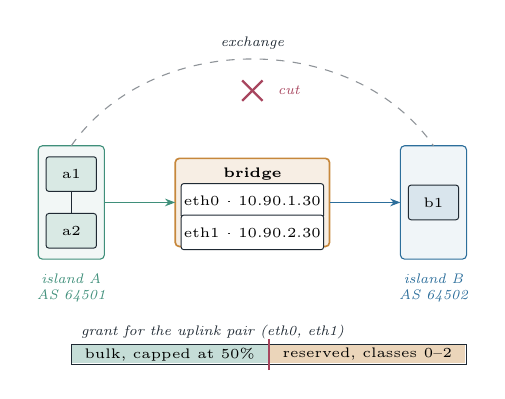
\begin{tikzpicture}[
  font=\scriptsize,
  nd/.style={draw=jbInk,line width=0.35pt,rounded corners=1pt,
             minimum width=6.4mm,minimum height=4.4mm,inner sep=1pt,font=\tiny},
  lbl/.style={font=\tiny\itshape,text=jbInk},
  >={Stealth[length=1.3mm]}
]
% island A
\draw[draw=jbTeal,line width=0.4pt,rounded corners=1.5pt,fill=jbTeal!7]
  (-0.42,-0.72) rectangle (0.42,0.72);
\node[nd,fill=jbTeal!20] (a1) at (0,0.36) {a1};
\node[nd,fill=jbTeal!20] (a2) at (0,-0.36) {a2};
\draw[jbInk,line width=0.3pt] (a1) -- (a2);
\node[lbl,text=jbTeal,anchor=north,align=center] at (0,-0.78) {island A\\AS 64501};
% bridge
\draw[draw=jbAmber,line width=0.6pt,rounded corners=1.5pt,fill=jbAmber!14]
  (1.32,-0.56) rectangle (3.28,0.56);
\node[font=\tiny\bfseries] at (2.3,0.36) {bridge};
\node[nd,fill=white,minimum width=13mm] (u1) at (2.3,0.02) {eth0 \textperiodcentered\ 10.90.1.30};
\node[nd,fill=white,minimum width=13mm] (u2) at (2.3,-0.38) {eth1 \textperiodcentered\ 10.90.2.30};
% island B
\draw[draw=jbBlue,line width=0.4pt,rounded corners=1.5pt,fill=jbBlue!7]
  (4.18,-0.72) rectangle (5.02,0.72);
\node[nd,fill=jbBlue!18] (b1) at (4.6,0) {b1};
\node[lbl,text=jbBlue,anchor=north,align=center] at (4.6,-0.78) {island B\\AS 64502};
\draw[-{Stealth[length=1.3mm]},jbTeal,line width=0.45pt] (0.42,0) -- (1.32,0);
\draw[-{Stealth[length=1.3mm]},jbBlue,line width=0.45pt] (3.28,0) -- (4.18,0);
% severed exchange
\draw[dashed,jbInk!50] (0,0.72) to[out=55,in=125] node[pos=0.5,above,lbl]{exchange} (4.6,0.72);
\coordinate (x) at (2.3,1.42);
\draw[jbRose,line width=0.8pt] ($(x)+(-1.3mm,-1.3mm)$) -- ($(x)+(1.3mm,1.3mm)$);
\draw[jbRose,line width=0.8pt] ($(x)+(1.3mm,-1.3mm)$) -- ($(x)+(-1.3mm,1.3mm)$);
\node[lbl,text=jbRose,anchor=west] at ($(x)+(2mm,0)$) {cut};
% quota split
\begin{scope}[shift={(0,-2.06)}]
  \node[lbl,anchor=west] at (0,0.42) {grant for the uplink pair (eth0, eth1)};
  \draw[draw=jbInk,line width=0.3pt] (0,0) rectangle (5.02,0.26);
  \fill[jbTeal!30] (0.015,0.015) rectangle (2.51,0.245);
  \fill[jbAmber!35] (2.51,0.015) rectangle (5.005,0.245);
  \draw[jbRose,line width=0.5pt] (2.51,-0.07) -- (2.51,0.33);
  \node[font=\tiny] at (1.25,0.13) {bulk, capped at 50\%};
  \node[font=\tiny] at (3.76,0.13) {reserved, classes 0--2};
\end{scope}
\end{tikzpicture}
\caption{The partition testbed, which is also the bridging mechanism. The islands occupy separate
address spaces on networks declared internal, so once the exchange is cut no route exists between them
except through the bridge. The bridge binds each outbound connection to the matching uplink's source
address, which we confirm by reading \texttt{/proc/net/tcp} inside the running container. Quota is
accounted per uplink \emph{pair}, and bulk draws on a bucket capped at half the grant so a forum
backlog cannot starve an emergency broadcast.}
\label{fig:testbed}
\Description{Two nodes in ISP island A and one node in ISP island B communicate only through a bridge
with one source-bound interface on each island after their direct exchange is cut.}
\end{figure}

\paragraph{Measurement boundary.} Host contention confounded a drain-interval sweep, so we report one
clean configuration rather than a parameter effect we could not isolate. Propagation uses the storage
timestamps written with each projection. Container clocks are shared; a field deployment would need
clock discipline and an error bound.

\subsection{Cross-implementation agreement}
\label{sec:eval-vectors}

The admission gate of \S\ref{sec:canonical} only works if the accepted encoding is genuinely agreed
across implementations. Otherwise it turns into a compatibility bug that rejects honest peers. Three
independent implementations of the canonical encoder, in TypeScript, Rust and Python, each written
against the specification rather than ported from one another, agree byte for byte on all 16
conformance vectors, covering field omission, NFC normalisation, domain separation and plane
separation. This is what makes strictness affordable, and it is our answer to the natural objection
that two implementations will eventually disagree.

\subsection{Correctness under partition}

Across independent datastores, both nodes project the same post and origin-derived community
identifier. Rebuilding every collection from the envelope log reproduces it byte for byte. The client
also rejects a wrong receipt key, a tree head that omits the content and a content identifier copied
from another envelope. The federation suite covers 31 assertions across admission, quota, streaming,
backfill, fork detection and directory exchange.

\subsection{Multi-hop propagation}

Figure~\ref{fig:hops} reports an eight-node chain, 200 paced samples, with a 1000\,ms outbox drain
interval. All 200 envelopes reached hop~7, and the seven-hop median is 4125\,ms against a p99 of
6115\,ms.
\begin{figure}[t]
\centering
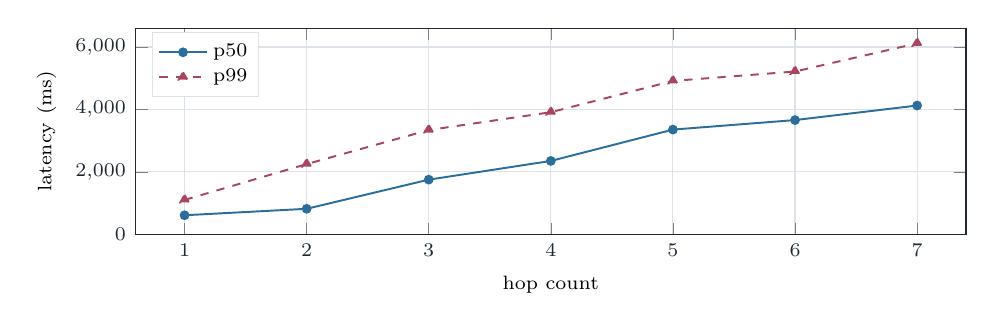
\begin{tikzpicture}
\begin{axis}[
  width=\columnwidth, height=42mm,
  font=\scriptsize,
  xlabel={hop count}, ylabel={latency (ms)},
  xlabel near ticks, ylabel near ticks,
  xmin=0.6, xmax=7.4, ymin=0, ymax=6600,
  xtick={1,2,3,4,5,6,7},
  ytick={0,2000,4000,6000},
  grid=major, grid style={jbMist},
  axis line style={jbInk}, tick label style={text=jbInk},
  legend style={at={(0.02,0.98)},anchor=north west,draw=jbMist,
                font=\scriptsize,row sep=-1pt,inner sep=2pt},
  legend cell align=left
]
\addplot[jbBlue,mark=*,mark size=1.4pt,line width=0.7pt]
  coordinates {(1,613)(2,820)(3,1753)(4,2352)(5,3355)(6,3660)(7,4125)};
\addlegendentry{p50}
\addplot[jbRose,mark=triangle*,mark size=1.8pt,line width=0.7pt,dashed]
  coordinates {(1,1104)(2,2251)(3,3341)(4,3912)(5,4913)(6,5215)(7,6115)};
\addlegendentry{p99}
\end{axis}
\end{tikzpicture}
\caption{Propagation latency by hop count. Eight-node chain, 200 paced samples, zero loss: all 200
envelopes reached hop~7. Growth is linear in hop count, and the outbox drain interval sets the slope,
not the protocol.}
\label{fig:hops}
\Description{A line chart showing median and ninety-ninth percentile propagation latency increasing
with hop count; all two hundred envelopes reach the seventh hop.}
\end{figure}

Per-hop cost is set by the drain interval, not by the protocol. Predicting
$\textit{drain}/2 + \textit{fixed}$ and measuring at two operating points isolates the constant. At a
1000\,ms drain the seven-hop median implies 589\,ms per hop and a fixed residual of 89\,ms; at 250\,ms
it implies 196\,ms per hop and a residual of 71\,ms. The residual holds at \textbf{71--89\,ms across a
fourfold change in the queueing parameter}, and it is the protocol's real per-hop cost: verify,
project, append to the witness log, re-enqueue. Everything above it is a scheduling choice an operator
makes for battery and bandwidth reasons.

\textbf{We report the offered-load regime with every figure, because it dominates the result.}
Publishing the same 200 envelopes as fast as the origin would accept them produced a first-hop median
of 10.0\,s and a 95th percentile of 173\,s, while the \emph{marginal} cost of hops 2--7 stayed at
0.4--1.1\,s. That shape is queueing and contention on a shared database, not propagation. Both are
correct measurements of different questions, and averaging them would describe neither.

\subsection{Bridged crossing}

Crossing an ISP boundary is not one envelope. A newly published post that a receiving island can
render depends on the author's certificate and on the community record, so three envelopes have to
cross and project in dependency order (Figure~\ref{fig:crossing-sequence}).

\begin{figure}[t]
\centering
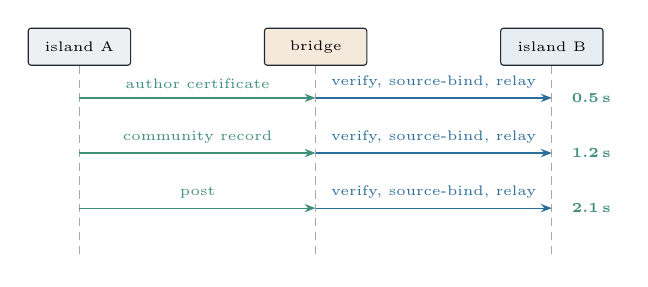
\begin{tikzpicture}[
  font=\tiny,
  actor/.style={draw=jbInk,fill=jbMist!55,rounded corners=1pt,minimum width=13mm,
                minimum height=4.7mm,align=center},
  >={Stealth[length=1.4mm]}
]
\node[actor] (a) at (0,0) {island A};
\node[actor,fill=jbAmber!18] (br) at (3.0,0) {bridge};
\node[actor,fill=jbBlue!12] (b) at (6.0,0) {island B};
\draw[densely dashed,jbInk!40] (a.south) -- ++(0,-2.45);
\draw[densely dashed,jbInk!40] (br.south) -- ++(0,-2.45);
\draw[densely dashed,jbInk!40] (b.south) -- ++(0,-2.45);
\foreach \y/\label/\time in {-0.65/author certificate/0.5\,s,-1.35/community record/1.2\,s,-2.05/post/2.1\,s}{
  \draw[->,jbTeal,line width=0.45pt] (0,\y) -- node[above]{\label} (3.0,\y);
  \draw[->,jbBlue,line width=0.45pt] (3.0,\y) -- node[above]{verify, source-bind, relay} (6.0,\y);
  \node[anchor=west,text=jbTeal,font=\tiny\bfseries] at (6.13,\y) {\time};
}
\end{tikzpicture}
\caption{The measured dependency chain after the exchange is cut. The far island can render the post
only after its author certificate and community record arrive first.}
\label{fig:crossing-sequence}
\Description{Three envelopes cross from island A through a verifying bridge to island B. The author
certificate arrives after 0.5 seconds, the community record after 1.2 seconds and the post after 2.1 seconds.}
\end{figure}

The cut-path arrivals are 0.5, 1.2 and 2.1\,s; the healthy-path figures are 1.5, 1.5 and 1.9\,s.
Once traffic uses the bridge, the cut does not meaningfully slow this crossing. The container gate
also passes source binding, directional accounting, reserved capacity and uplink failover.

Inside the bridge, \texttt{/proc/net/tcp} confirms sockets leave from both configured source
addresses, an assertion an in-process harness cannot make.

The first deployed run took 407.6\,s: a serial, deadline-free drain blocked on one blackholed peer,
so the bridge behind it was never attempted. Concurrent per-peer drains with deadlines restored the
2.1\,s crossing. Multi-homing is defeated if a node inherits its worst peer's availability.

\subsection{An invalid-envelope flood does not become write load}
\label{sec:flood}

We flooded a node with well-formed, unique envelopes whose signed region had one mutated byte. Unlike
random bytes, these reach the costly checks and cannot be removed by deduplication.

Against a single node, 3000 such envelopes at concurrency~16 were absorbed at \textbf{730\,req/s}, and
the node's database recorded \textbf{zero writes}. The envelope log was unchanged, and a
collection-level profiler logged no insert, update or delete while still capturing read operations
over the same window, which confirms it was live. Resident memory fell from 86\,MiB to 61\,MiB as the
garbage collector caught up, and CPU returned to idle immediately.

Only 9\% reached signature verification; \textbf{90\% was shed by the per-peer rate limiter}. The
no-write prefix is therefore the second line of defence, not the source of all measured throughput.

\paragraph{A defect surfaced.} Eight requests initially returned HTTP 500 because metric labelling
decoded untrusted bytes outside the pipeline and emitted stack traces. The label now falls back to a
constant, four adversarial encodings have regression tests, and rejection rose from 440 to 730\,req/s.

\subsection{Read path and footprint}

The keep-alive read path peaks at 750\,req/s (concurrency~8). An idle node uses 62\,MiB RSS and
233\,MiB under sustained crossing; node, database and cache together use roughly 384\,MiB of a
512\,MB target. Storage is the binding constraint on small hardware.

\subsection{Encoded size against a measured ActivityPub baseline}

Encoded envelopes including a 64-byte signature are 155\,B for a check-in, 220\,B for a forum post
and 243\,B for a Bangla broadcast. We compare them with 80 real \texttt{Create}/\texttt{Note}
activities from two stock ActivityPub instances, re-attaching each host's JSON-LD context as remote
delivery does.
\begin{table}[t]
\caption{Encoded size, ours against 80 real ActivityPub activities. Overhead leaves out authored
text, which is a confound: our fixture carries a 14-character headline, while the sampled posts carry
30--524\,B.}
\label{tab:size}
\small
\begin{tabular}{lrrr}
\toprule
 & p50 & min & max \\
\midrule
ActivityPub delivered (B)      & 4216 & 2786 & 6909 \\
\quad of which authored text   &  205 &   30 &  524 \\
\quad of which JSON-LD context &  927 &  927 &  927 \\
\textbf{ActivityPub overhead (B)} & \textbf{4015} & 2756 & 6484 \\
ActivityPub, gzipped (B)       & 1074 &  786 & 1400 \\
\midrule
Ours, check-in / post / broadcast (B) & \multicolumn{3}{r}{155 / 220 / 243} \\
\textbf{Ours, overhead (B)}    & \multicolumn{3}{r}{\textbf{155 / 206 / 177}} \\
\bottomrule
\end{tabular}
\end{table}

After subtracting authored text, ActivityPub's overhead is \textbf{19.5$\times$--25.9$\times$}
ours; its 927\,B context alone is 4.2 times our signed post. Compression narrows this to
\textbf{4.4$\times$--6.9$\times$}: signatures do not compress and gzip makes our envelopes larger.
We omit HTTP framing and ActivityPub authentication, and count one activity rather than follower
fanout. JSON-LD also buys extensibility our fixed schema does not; the table measures link bytes only.

%% ---------------------------------------------------------------------------
\section{Comparison with Related Systems}
\label{sec:comparison}

No quantitative baseline exists for ``keeps a public forum readable across an ISP partition'', so we
compare capabilities. Table~\ref{tab:matrix} scores the signed-content publishing systems that are
genuine peers --- every one of them has a checkable specification --- on the ladder and on the
integrity properties this design turns on. We checked every cell against the system's own
specification.

\begin{table}[t]
\caption{Capability comparison. \CIRCLE~provided and specified, \LEFTcircle~partial, optional or
non-normative, \Circle~not provided. \textsc{nf}~indicates the specification is silent. \emph{No
inbound}: a node with no reachable address still participates in both directions. \emph{Svr}: the
specification defines a server-to-server exchange at all. ActivityPub's partial score reflects
measured hosting concentration and graph-removal analysis, not a protocol partition test~\cite{raman2019mastodon}.}
\label{tab:matrix}
\scriptsize
\setlength{\tabcolsep}{3.4pt}
\begin{tabular}{lcccccccc}
\toprule
 & L0--L3 & no in- & signed & verify & no re- & log & tomb- & svr \\
 & span & bound & at rest & w/o srv & encode & gossip & stone & $\leftrightarrow$srv \\
\midrule
ActivityPub        & \LEFTcircle & \Circle & \LEFTcircle & \Circle & \Circle & \Circle & \LEFTcircle & \CIRCLE \\
Netnews            & \LEFTcircle & \Circle & \Circle     & \Circle & \textsc{nf} & \Circle & \LEFTcircle & \CIRCLE \\
Matrix             & \LEFTcircle & \Circle & \CIRCLE     & \CIRCLE & \Circle & \Circle & \CIRCLE     & \CIRCLE \\
AT Protocol        & \Circle     & \Circle & \CIRCLE     & \LEFTcircle & \CIRCLE & \Circle & \Circle & \CIRCLE \\
Nostr              & \LEFTcircle & \CIRCLE & \CIRCLE     & \CIRCLE & \LEFTcircle & \Circle & \Circle & \LEFTcircle \\
Secure Scuttlebutt & \LEFTcircle & \CIRCLE & \CIRCLE     & \CIRCLE & \textsc{nf} & \Circle & \Circle & \CIRCLE \\
\textbf{This work} & \CIRCLE     & \CIRCLE & \CIRCLE     & \CIRCLE & \CIRCLE & \CIRCLE & \CIRCLE & \CIRCLE \\
\bottomrule
\end{tabular}
\end{table}

Secure Scuttlebutt is stronger below L1: local broadcast discovery needs no configured infrastructure,
whereas our lowest measured rung needs a multi-ISP operator. Nostr obtains no-inbound participation
from its client-pull architecture. Server-to-server exchange itself is common, not novel.

ActivityPub scores \LEFTcircle\ on tombstoning because Activity Streams defines the type, but does not
require it to remain publicly retrievable~\cite{activitystreams}. AT Protocol scores \LEFTcircle\ on
offline verification: a cached DID key verifies an object, while a current key binding needs DID
resolution~\cite{atproto,balduf2024bluesky}.

No column here is novel on its own. What no prior system holds is the \emph{conjunction} of
server-to-server reach, participation without inbound reachability, and gossiped log heads, while
spanning L0--L3 --- and what this paper reports is the engineering cost of that combination rather
than its novelty.

%% ---
%% ---------------------------------------------------------------------------
\section{Limitations}
\label{sec:limitations}

\textbf{One-host containers are a confound.} Clocks are aligned, networks are virtual and nodes share
storage. A repeated configuration changed first-hop median fivefold, so chain length and queueing
remain unswept and there is no wide-area or lossy-link measurement.

\textbf{A severed virtual bridge is not a field trial.} Route removal reproduces lost reachability,
not DPI, selective throttling or coercion. The partition result is a lower bound on mechanism cost.

\textbf{Unlinkability is architectural, not proven.} The separation between identity planes has no
formal argument and no anonymity-set analysis, and we make no claim of resistance to a global passive
observer.

\textbf{One operator configured every node.} Probation, vouching, demotion and governance remain
unobserved between strangers.

\textbf{Complementary transports and the Signal plane are not evaluated here.} The implementation
includes Tor client access, local WebRTC exchange, offline bundles, a separate identified Signal
plane and an optional Reticulum sidecar. None contributes to the L0--L3 measurements. We have not
measured Tor bootstrap or blocking resistance, local peer exchange, radio delivery, encrypted
messaging or crisis-report usability under interference.

\textbf{The open-taxonomy labelling extension (\S\ref{sec:classify}) is specified, not measured.}
No classifier is deployed against it and no client renders a capability manifest; nothing in
\S\ref{sec:eval} reflects it, and the claim made for it is only that it reuses the write path
unchanged.

%% ---------------------------------------------------------------------------
\section{Conclusion}
Availability under partition is a design ordering, not a feature. Putting it first forces
specific and sometimes uncomfortable choices: identifiers derived from signed bytes rather than from
the node that stores them, admission cost charged once at the origin rather than re-verified on
receipt, canonical encoding used to admit rather than to verify, and a rejection where a more
forgiving system would repair. We have shown that this composition works from global reach down to
bridged ISP islands, measured what it costs in latency, memory and bytes, and reported an
availability defect that only a deployed multi-peer testbed could expose. What we have not done is
run it during a real shutdown, under a real adversary, between operators who are strangers to each
other. That is the measurement the design is actually asking for, and it is the work we think matters
next.
\bibliographystyle{ACM-Reference-Format}
\bibliography{references}

\end{document}
